\chapter{Propiedades calculadas}

En este capítulo se describen las ecuaciones y los métodos usados para extraer resultados del sistema estudiado. En particular describimos la función de distribución radial, el número de coordinación, coeficiente de difusión,  la temperatura, energía y presión. Al final de este capítulo se detalla el sistema simulado.

\section{Función de distribución radial y número de coordinación}
% \textcolor{red}{usar mejor la definición de VMD para enlazar bien el marco teórico con la metodología}

Esta función es importante ya que proporciona información estructural promedio del sistema.\\

Esta función da la probabilidad de encontrar un par de átomos a distancia r, relativa a la probabilidad de una distribución completamente aleatoria a la misma densidad. En la dinámica molecular, la función de distribución radial se calcula usando la relación (\ref{gr})\\

\begin{equation} \label{gr}
    g(r)=\lim_{dr\to 0} \frac{\left<N(r, r+dr)\right>}{\frac{4 \pi}{3} \rho \left[(r+dr)^3 - r^3\right]}
\end{equation}\\

\noindent donde $r$ es la distancia entre átomos, $\left<N(r, r+dr)\right>$ es el número promedio de átomos encontrados a una distancia entre $r$ y $r + dr$, $\rho$ es la densidad total del sistema.

El promedio $\left<N(r, r+dr)\right>$ es calculado sobre toda la trayectoria de una simulación.

\begin{figure}[!h]
    \centering
    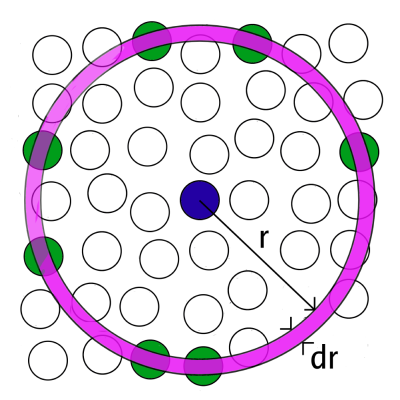
\includegraphics[width=.2\textwidth,keepaspectratio=true]{gr.png}
    \caption{Evaluación de la función de distribución radial}
    \label{fig:gr}
\end{figure}

% \begin{equation} \label{gr}
%     g(r)=\lim_{dr\to 0} \frac{p(r)}{4\pi \left(N_{pares}/V\right)r^{2}dr}
% \end{equation}\\

% donde $r$ es la distancia entre átomos, $p(r)$ es el promedio del número de pares de átomos encontrados a una distancia entre $r$ y $r+dr$, V el volumen total del sistema y $N_{pares}$ es el número de pares únicos de átomos donde un átomo es de cada uno de dos conjuntos, $sel_1$ y $sel_2$.\\

% \begin{figure}[!h]
%     \centering
%     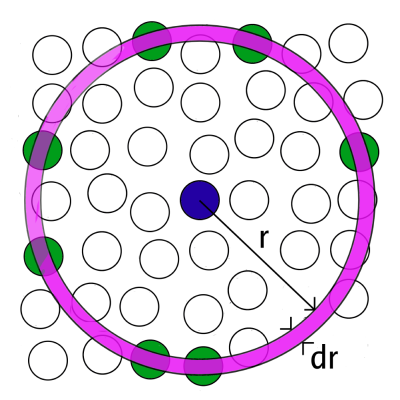
\includegraphics[width=.2\textwidth,keepaspectratio=true]{gr.png}
%     \caption{Evaluación de la función de distribución radial}
%     \label{fig:gr}
% \end{figure}

% El promedio $p(r)$ es calculado sobre toda la trayectoria de una simulación con $N_{cuadros}$ el número total de cuadros en la simulación. Este promedio toma la forma de:\\

% \begin{equation}\label{p}
%     p(r)=\frac{1}{N_{cuadros}}\sum^{N_{cuadros}}_i \sum_{j\in sel1} \sum_{k\in sel2} \sum_{\kappa} d_{\kappa}(r_{ijk})
% \end{equation}\\

% donde $\kappa$ son los índices de los contenedores del histograma y

% \begin{equation}
%     d_{\kappa}(r_{ijk}) = 
%     \begin{cases}
%         1 / \Delta r &\text{si $r_\kappa \leqq r<r_\kappa + \Delta r$ y $r_\kappa \leqq r_{ijk}<r_\kappa + \Delta r$}\\
%         0 & \text{de otra manera}\\
%     \end{cases}
% \end{equation}

% donde $\Delta r$ es el ancho de los contenedores del histograma y $r_\kappa$ es la distancia mínima asociada con cada contenedor, dado por:

% \begin{equation}
%     r_\kappa = r_0 + \kappa \Delta r
% \end{equation}

% con $r_0$ el límite inferior del histograma.\\

% El cálculo de la función de distribución radial también cumple con la convención de mínima imagen. El límite superior del histograma debería no ser mayor a $L/2$.\\

El número de coordinación se calcula como

\begin{equation}
    N(r) =  \int_0^{r_m} \rho g(r)4\pir^{2}dr
\end{equation}

\noindent donde $r_m$ es la distancia en que se encuentra el primer mínimo de $g(r)$ y $\rho$ es la densidad de bulto del sistema. Este es un promedio del número de vecinos hasta $r_m$ \cite{GOCHENOUR201841}. Para el caso de la simulación, es el promedio en todos los cuadros.\\

\section{Propiedades macroscópicas del sistema}

\subsection{Energía}

El promedio de la energía se calcula como el promedio de la ecuación (\ref{hamiltoniano}) \cite{Allen2017}:

\begin{equation} \label{promenergia}
    \langle E \rangle = \left \langle\sum_{i=1}^{N} \frac{1}{2 m_i}\dot{\mathbf{p}}_i^2 \right \rangle+ \left \langle\sum_{i=1}^{N-1}\sum_{j=i+1}^{N} u(r_{ij})\right \rangle
\end{equation}

\subsection{Temperatura}

Aunque la temperatura se mantiene fija en la simulación proporcionamos su descripción \cite{Allen2017}.

\begin{equation} \label{virialtheorem}
    \left \langle p_k \frac{\partial H}{\partial p_k} \right \rangle = k_B T.
\end{equation}

Para el hamiltoniano en la ecuación (\ref{hamiltoniano}) encontramos:

\begin{equation} \label{virialtemp}
    k_B T = \left \langle p_k \frac{p_k}{m_k} \right \rangle
\end{equation}

\noindent entonces derivamos la siguiente ecuación al incorporar la suma para los 3N términos de N partículas:

\begin{equation} \label{virialsumtemp}
    3Nk_B T = \left \langle \sum_{k=1}^{N}\frac{|p_k|^2}{m_k} \right \rangle.
\end{equation}

Para un sistema donde hay $N_C$ restricciones de algún tipo (e.g. descripciones de centro de masa, ángulos rígidos, enlaces rígidos entre otros), la ecuación anterior se convierte en:

\begin{equation} \label{virialsumconsttemp}
    T= \frac{1}{3(N - N_C)k_B}\left \langle \sum_{k=1}^{N}\frac{|p_k|^2}{m_k} \right \rangle
\end{equation}

\subsection{Presión}

% La otra ecuación del teorema del virial nos da la siguiente ecuación:

% \begin{equation} \label{virialtheoremq}
%     \left \langle q_k \frac{\partial H}{\partial q_k} \right \rangle = k_B T
% \end{equation}

% lo cual nos lleva a:

% \begin{equation} \label{virialtheorempress}
%     \frac{1}{3}\left \langle \sum_{i=1}^N \mathbf{r_i} \cdot \mathbf{f}^{tot}_i \right \rangle = -N k_B T
% \end{equation}

% si dividimos la fuerza total entre externa e intermolecular llegamos a otra ecuación \cite{Allen2017}:

La presión promedio se determina considerando su contribución cinética y la parte debida a interacciones, a través de

\begin{equation} \label{virialsumconstpress}
    P = \frac{N}{\left \langle V \right \rangle} k_B T + \frac{\left \langle \mathcal{W} \right \rangle}{\left \langle V \right \rangle}
\end{equation}

\noindent donde $\mathcal{W} = \frac{1}{3} \sum_{i=1}^N \mathbf{r_i} \cdot \mathbf{f}_i$ con $\mathbf{f}_i$ fuerzas intermoleculares las cuales se obtienen a través del campo de fuerzas.

\section{Coeficiente de difusión}

% La ecuación de difusión describe como alguna variable se propaga en un sistema, por ejemplo, unir una barra metálica caliente con otra fría (conocida como la ecuación de difusión de calor).

% La difusión molecular puede interpretar como dos sistemas con diferentes temperaturas o variable termodinámica fluye hacia el equilibrio.

% Por la naturaleza molecular de un sistema, se puede modelar las interacciones de las moléculas como una caminata aleatoria(así ignoramos la interacción o la implicación de momentos, fuerzas, entre otros).

% Podemos hacer primero un modelo de esta caminata aleatoria de manera discreta en el espacio y tiempo hasta llevarlo de manera continua en espacio y tiempo tomando en cuenta el promedio del movimiento de partículas

% Primero describimos el modelo aleatorio en una dimensión. En una sección de recta numérica dejamos como ejemplo mil partículas (con distribución de 50-50 de moverse a ambos lados) distribuidas de igual manera a la mitad del lado izquierdo con una condición de frontera que si una partícula se encuentra en alguna de las frontera, su probabilidad es 50% y 50% en quedarse en el mismo lugar o moverse contrario a la frontera.

%En promedio mitad de la densidad lineal de partículas en un i-esimo delta x se movera hacia la izquierda y la otra mitad a la derecha y la mitad de la densidad lineal de los vecinos entrará

% En ecuación esto es, delta rho_i = 1/2[(rho_{i+1}-rho_{i})-(rho_{i}-rho_{i-1})]

% La constante de difusión da la idea de que tan rápido se mueven las partículas

Los coeficientes de transporte como el coeficiente de difusión describen la relajación de variables dinámicas en la escala macroscópica. Siempre considerando que el tiempo y los límites a gran escala son los adecuados, pueden ser descritos en términos de funciones de correlación de tiempo en equilibrio microscópicos \cite{Allen2017}. Para un sistema en equilibrio, el coeficiente de difusión de las partículas de tipo A, $D_A$, se obtiene a través de \cite{gromacsdoc}

\begin{equation} \label{diffusioncoeff}
    D_A = \frac{1}{6} \lim_{t \to \infty} \left\langle\left\| \mathbf{r}_{i}(t) - \mathbf{r}_{i}(0) \right\|^2 \right\rangle_{i \in A},
\end{equation}

\noindent es decir, el coeficiente de difusión está dado por el desplazamiento cuadrático medio del centro de masa de las posiciones de las moléculas. Este representa la movilidad de las moléculas en la solución, de igual manera que la conductividad eléctrica representa la de los electrones a través del material.\\

En el programa de simulación usado, se puede calcular el coeficiente de difusión de un grupo de moléculas o átomos \cite{gromacsdoc}.

\section{Sistema simulado}

El sistema se simuló en un rango de temperaturas de 280 a 370 K, que consta de 16807 moléculas de agua, 10 moléculas de ácido 2,4-diclorofenoxiacético (2,4-D) y un nanotubo de carbono (6, 5) con una longitud alrededor de 38nm. En todas las simulaciones se usó el termostato de Nosé-Hoover acoplado con un barostato Parrinello-Rahman con $\tau_t$ de 0.4 ps y $\tau_p$ de 1.6 ps, respectivamente.\\

Todas las simulaciones constaron de 20 ns de tiempo de simulación, se usó el algoritmo de salto de rana y radio de corte de 1.2 nm. La validez de los parámetros del termostato y barostato fue verificada revisando que las condiciones de simulación fueron mantenidas de manera adecuada conforme los valores impuestos en la simulación NPT, como se muestra en la tabla \ref{tab:promediostemppres}.

\begin{table}[h!]
    \centering
    \begin{tabular}{ |m{6em}|m{5em}||m{5em}|m{5em}|  }
    \hline
    Temperatura (K) & Error & Presión (bar) & Error \\
    \hline
    \hline
    280.003 & 0.0018 & 0.840079 & 0.12 \\
    298.149 & 0.0014 & 1.11589 & 0.099 \\
    309.998 & 0.0013 & 1.28056 & 0.2 \\
    319.996 & 0.0012 & 1.01285 & 0.12 \\
    329.998 & 0.0016 & 1.12986 & 0.079 \\
    340 & 0.0019 & 1.11812 & 0.13 \\
    349.998 & 0.0028 & 1.30148 & 0.13 \\
    360.003 & 0.0022 & 1.02411 & 0.13 \\
    370.002 & 0.002 & 1.1182 & 0.13 \\
    \hline
    \end{tabular}
    \caption{Promedio de temperatura y presión de los sistemas simulados. El error es calculado por el metodo de promedio de bloques \cite{gromacsdoc}.}
    \label{tab:promediostemppres}
\end{table}


% y el campo de fuerzas usado en el sistema es GROMOS 54A7, que tiene la siguiente forma en nuestras simulaciones:
% \begin{itemize}
%     \item Número de moléculas: 16807 moléculas de agua, 10 moléculas de ácido 2,4-diclorofenoxiacético (2,4-D) y un nanotubo de carbono (6, 5) con 364 átomos.
%     \item Integrador de todos los sistemas: salto de rana para las ecuaciones de movimiento de Newton.
%     \item Paso de tiempo: 0.002 ps, número de pasos: 10000000, Intervalo de tiempo: 20 ns.
%     \item radio de corte para la lista de vecinos de corto alcance: 1.2 nm, radio de corte para interacción de coulomb: 1.2 nm, radio de corte para interacción LJ 12-6: 1.2 nm.
%     \item Corrección de dispersión de largo alcance para energía y presión.
%     \item Acoplamiento de temperatura: ensamble extendido de nose-hoover con $\tau_t$: 0.4 ps y con las temperaturas antes mencionadas.
%     \item Acoplamiento de presión: ensamble extendido de parrinello-rahman con $\tau_p$: 1.6 ps a presión: 1 bar.
%     \item Algoritmo de constricción: LINCS(LINear Constraint Solver).
% \end{itemize}




